\appendix
\renewcommand{\thefigure}{S\arabic{figure}}
\renewcommand{\thetable}{S\arabic{table}}
\setcounter{figure}{0}
\setcounter{table}{0}
\section{Supplementary tables and figures}
\subsection{Decision tree and AdaBoost}\label{ap:decision_adaboost}
\begin{table}[h!]
    \centering
    \begin{tabular}{cc}
        \hline
        Index \, & Target \\
        \hline 
        $0$ & Acartia \\
        $1$ & Asplanchna \\
        $2$ & Chaetoceros single \\
        $3$ & Chaetoceros socialis Chaetoceros \\
        $4$ & Oithona \\
        $5$ & Pseudo-Nitzschia chain \\
        $6$ & Striatella \\
        $7$ & Thalassionema \\
        $8$ & Tintinnida \\
        $9$ & Tripos furca \\
        $10$ & Tripos fusus \\
        $11$ & Tripos muelleri \\
        $12$ & nauplii Copepoda \\
        $13$ & tintinnids empty \\
        \hline
    \end{tabular}
    \caption{Indices and species for the target data which the models were trained and tested on, when using metadata from the PlanktoScope}
    \label{tab:target_names}
\end{table}

\begin{table}[h!]
    \centering
    \begin{tabular}{cc}
        \hline
        Feature \, & Importance \\
        \hline 
        \verb|object_equivalent_diameter| & $0.1808$ \\
        \verb|object_perimareaexc| & $0.1712$ \\
        \verb|object_elongation| & $0.1407$ \\
        \verb|object_minor| & $0.1070$ \\
        \verb|object_eccentricity| & $0.0861$ \\
        \verb|object_extent| & $0.0707$ \\
        \verb|object_meanvalue| & $0.0626$ \\
        \verb|object_meansaturation| & $0.0424$ \\
        \verb|object_stdsaturation| & $0.0374$ \\
        \verb|object_label| & $0.0157$ \\
        \verb|object_perimmajor| & $0.0154$ \\
        \verb|object_major| & $0.0130$ \\
        \verb|object_solidity| & $0.0112$ \\
        \verb|object_bx| & $0.0090$ \\
        \verb|object_local_centroid_row| & $0.0054$ \\
        \verb|object_stdvalue| & $0.0046$ \\
        \verb|object_width| & $0.0044$ \\
        \verb|object_height| & $0.0043$ \\
        \verb|object_circex| & $0.0039$ \\
        \verb|object_stdhue| & $0.0037$ \\
        \verb|object_bounding_box_area| & $0.0028$ \\
        \verb|object_x| & $0.0019$ \\
        \verb|object_circ.| & $0.0017$ \\
        \verb|object_convex_area| & $0.0017$ \\
        \verb|object_euler_number| & $0.0016$ \\
        \verb|object_y| & $0.0008$ \\
        \verb|object_local_centroid_col| & $0.0$ \\
        \verb|object_area| & $0.0$ \\
        \verb|object_meanhue| & $0.0$ \\
        \verb|object_by| & $0.0$ \\
        \verb|object_angle| & $0.0$ \\
        \verb|object_%area| & $0.0$ \\
        \verb|object_perim.| & $0.0$ \\
        \verb|object_area_exc| & $0.0$ \\
        \hline
    \end{tabular}
    \caption{Features and their importance in the decision tree model's prediction, when trained and tested on metadata from the PlanktoScope. The values are rounded and sorted by importance.}
    \label{tab:dt_ft_imp}
\end{table}

\begin{table}[h!]
    \centering
    \begin{tabular}{cc}
        \hline
        Feature \, & Importance \\
        \hline 
        \verb|object_perimareaexc| & $0.1612$ \\
        \verb|object_x| & $0.0843$ \\
        \verb|object_equivalent_diameter| & $0.0780$ \\
        \verb|object_stdsaturation| & $0.0747$ \\
        \verb|object_area_exc| & $0.0706$ \\
        \verb|object_meansaturation| & $0.0492$ \\
        \verb|object_perimmajor| & $0.0427$ \\
        \verb|object_area| & $0.0397$ \\
        \verb|object_solidity| & $0.0382$ \\
        \verb|object_extent| & $0.0382$ \\
        \verb|object_minor| & $0.0357$ \\
        \verb|object_elongation| & $0.0354$ \\
        \verb|object_eccentricity| & $0.0350$ \\
        \verb|object_meanvalue| & $0.0202$ \\
        \verb|object_major| & $0.0191$ \\
        \verb|object_%area| & $0.0191$ \\
        \verb|object_label| & $0.0172$ \\
        \verb|object_y| & $0.0168$ \\
        \verb|object_angle| & $0.0153$ \\
        \verb|object_circ.| & $0.0115$ \\
        \verb|object_stdvalue| & $0.0112$ \\
        \verb|object_local_centroid_col| & $0.0109$ \\
        \verb|object_bounding_box_area| & $0.0108$ \\
        \verb|object_by| & $0.0089$ \\
        \verb|object_height| & $0.0088$ \\
        \verb|object_perim.| & $0.0077$ \\
        \verb|object_width| & $0.0067$ \\
        \verb|object_meanhue| & $0.0065$ \\
        \verb|object_circex| & $0.0058$ \\
        \verb|object_local_centroid_row| & $0.0049$ \\
        \verb|object_convex_area| & $0.0047$ \\
        \verb|object_bx| & $0.0046$ \\
        \verb|object_euler_number| & $0.0036$ \\
        \verb|object_stdhue| & $0.0025$ \\
        \hline
    \end{tabular}
    \caption{Features and their importance in the AdaBoost model's prediction, when trained and tested on metadata from the PlanktoScope. The values are rounded and sorted by importance.}
    \label{tab:adaboost_ft_imp}
\end{table}


\subsection{CNN}\label{ap:cnn}


\begin{figure*}
    \centering
    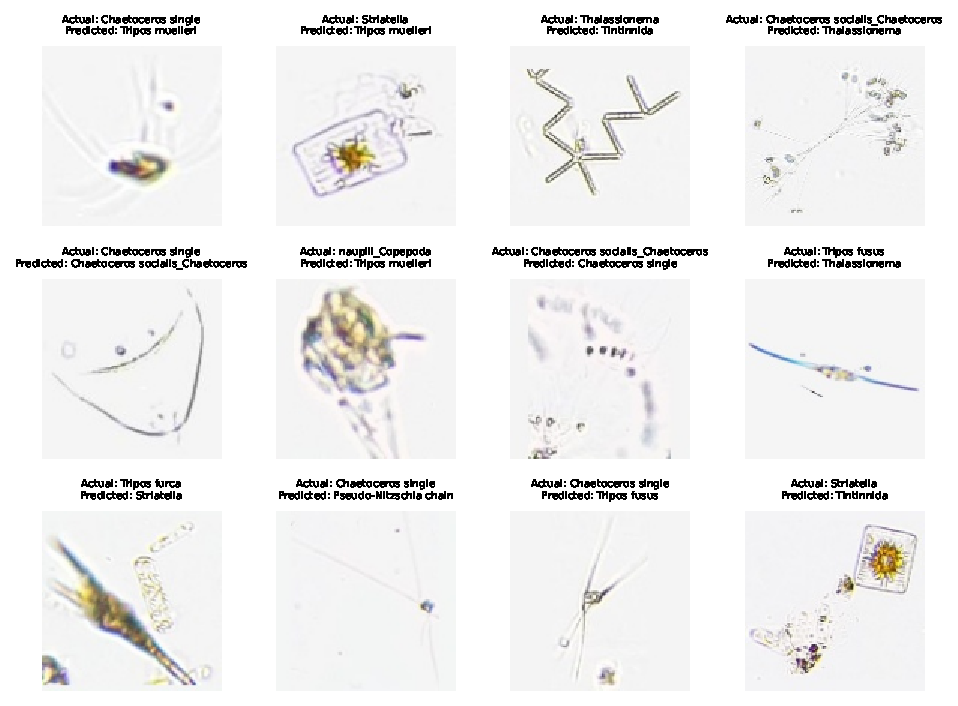
\includegraphics[width=0.8\linewidth]{examples/tests_even/figs/wrong-preds2-2024-12-06_1241.pdf}
    \caption{Caption}
    \label{fig:cnn-wrong-ps}
\end{figure*}

\begin{figure*}
    \centering
    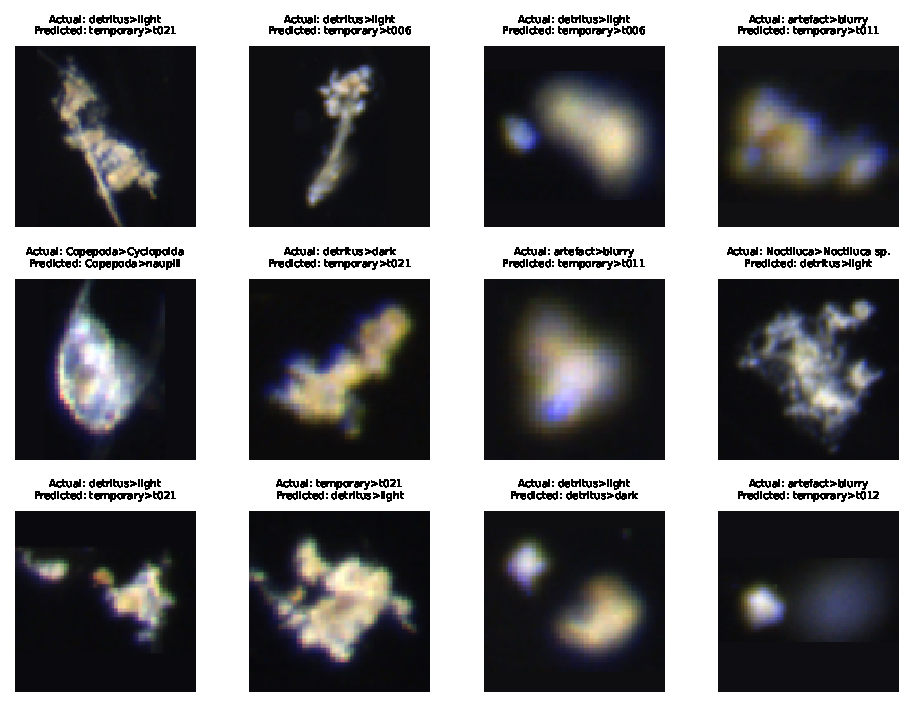
\includegraphics[width=0.8\linewidth]{examples/tests_even/figs/wrong-preds2-2024-12-09_1113.pdf}
    \caption{Caption}
    \label{fig:cnn-wrong-cpics}
\end{figure*}

\subsection{Dino}\label{ap:dino}
\begin{figure}[H]
    \centering
    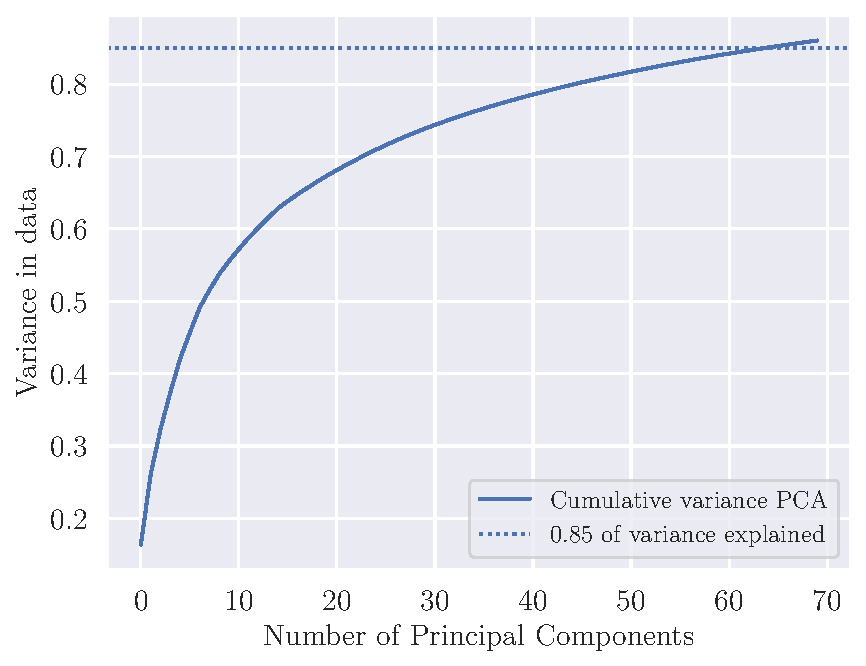
\includegraphics[width=0.9\linewidth]{examples/tests_eb/figs/cumsum_pca.pdf}
    \caption{A plot of the cumulative variance for each principal component included in our new, dimensionality reduced features. We concluded that 70 features was sufficient to capture just above 85 percent of the variance in our data.}
    \label{fig:cumsumpca}
\end{figure}

\begin{figure}[H]
    \centering
    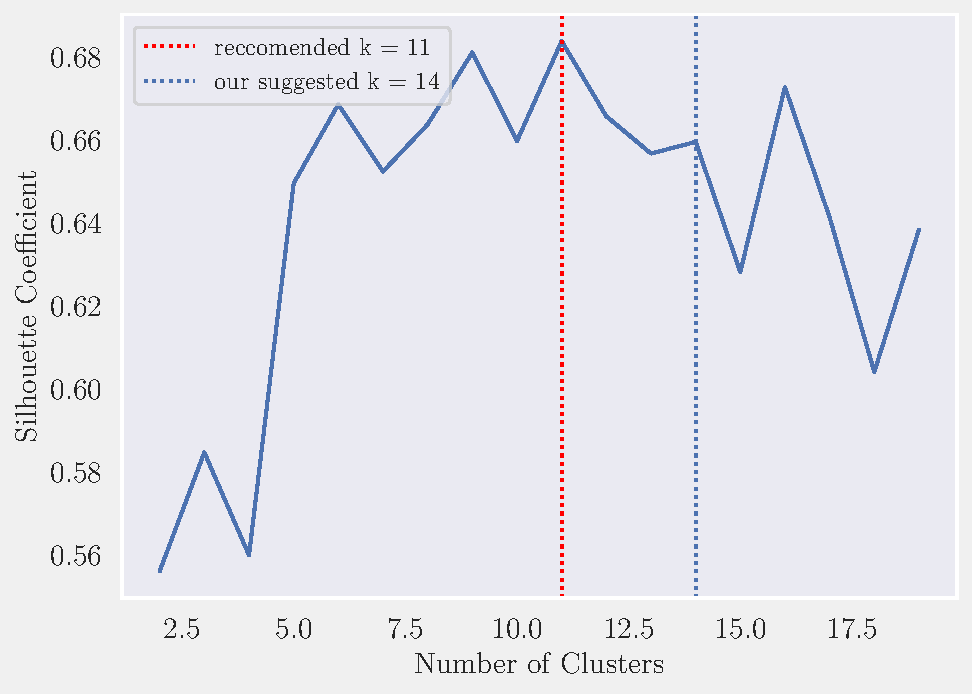
\includegraphics[width=0.9\linewidth]{examples/tests_eb/figs/kmean_sil.pdf}
    \caption{A plot of the silhouette scores for each KMean tested on UMAP data.}
    \label{fig_cumsumpca}
\end{figure}


\begin{figure}[H]
    \centering
    \begin{subfigure}[b]{1\linewidth}
        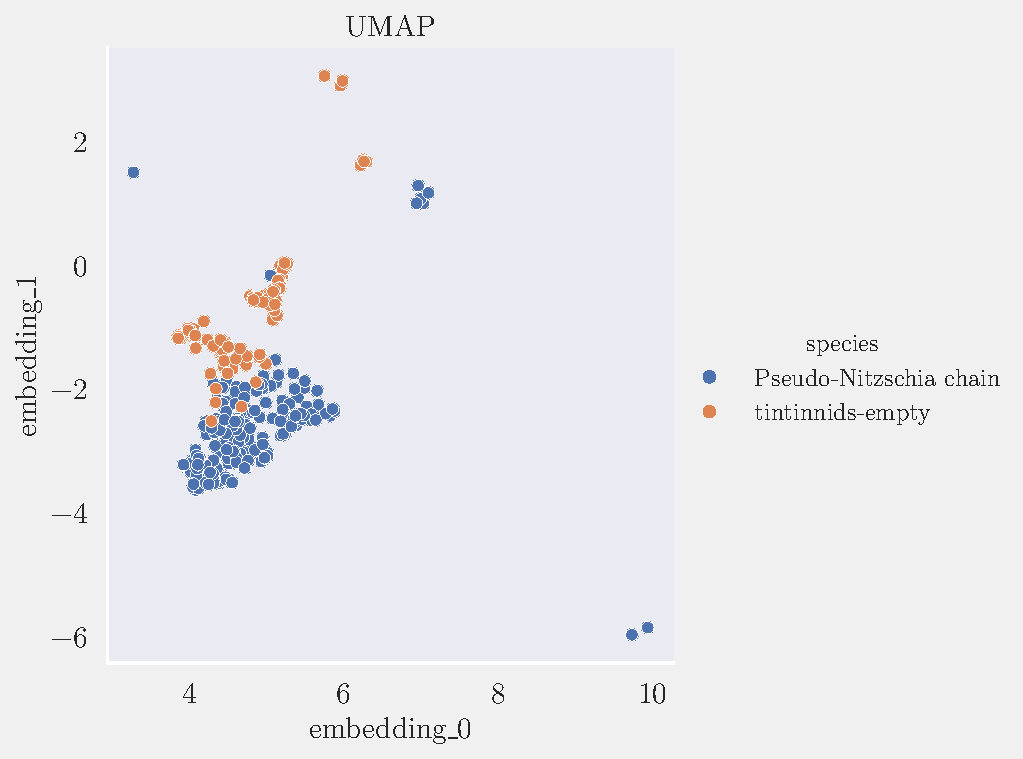
\includegraphics[width=\linewidth]{examples/tests_eb/figs/umap_on_two_species.pdf}
        \caption{First we isolated the already produced embeddings for the two species. Already here we can see that they form clysters according to their species.}
        \label{misclust1}
    \end{subfigure}
    
    \vspace{1em}
    
    \begin{subfigure}[b]{1\linewidth}
        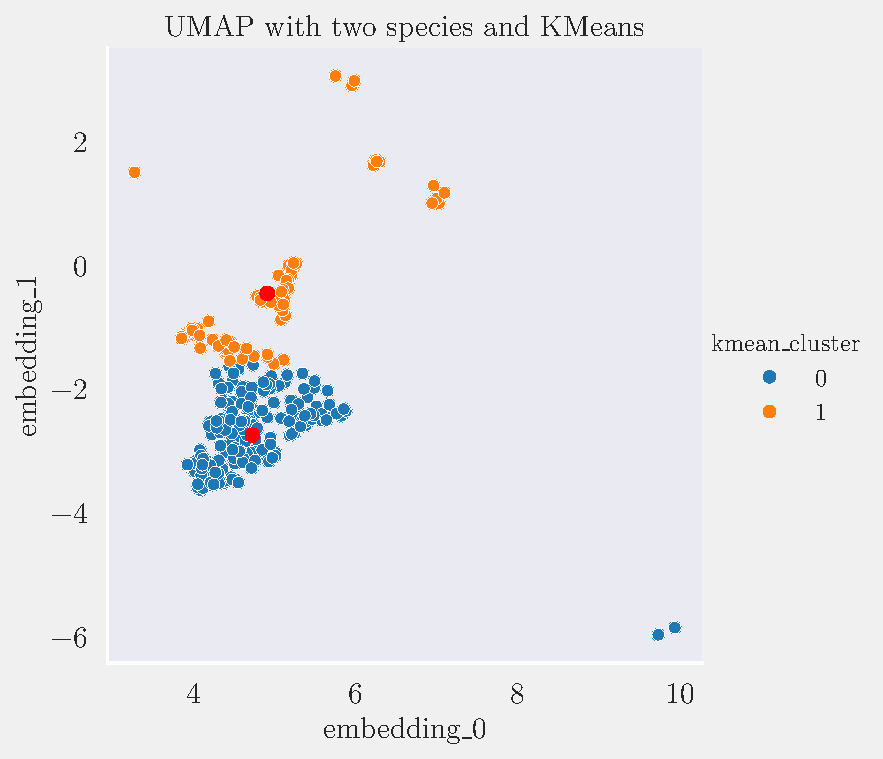
\includegraphics[width=\linewidth]{examples/tests_eb/figs/kmeans_cluster_umap_on_two_species.pdf}
        \caption{We performed a KMeans clustering with two clusters to find which images (or species) would cluster together in the embedding space. Red dots are kmer centroids.}
        \label{misclust2}
    \end{subfigure}
    \caption{The process of finding the images that misclustered in Figure \ref{fig:misclusters} explained. We display images of Pseudo N that were placed in cluster 1, and the opposite for Tintinnids-e.}
    \label{fig:misclustering_process}
\end{figure}
